\section{CPU usage}
\label{sec:cpu-usage}
	The anontunnels create a Tribler session, run multiple cryptographic functions and are relaying and downloading data. Each of these operations require CPU utilization. As mobile devices often have less resources than computers, we have to make sure that the CPU can handle the required operations.
	
	% FEEDBACK
	% Process CPU usage erbij zetten
	% Duidelijk uitleggen wat de grafiek is
	% Aanduidingen wanneer wat gebeurt (wanneer start tribler/dispersy? wanneer de app? etc)
	 % Alle grafieken hiervoor nagaan
	 % Hoe downloaden? Via libtorrent? Tribler?
	 % Verklaar pieken en dalen in de grafieken! Of "admit defeat" en dat we het niet kunnen verklaren.
	 % 1 duidelijk punt maken (je conclusie) met minder grafiekjes, misschien samenvoegen in 1 grafiek.
	 % 
	\subsection{CPU usage when idle}
		We first measured the CPU usage when the application is idle. The CPU usage is shown in figure \ref{fig:cpu_idle_graph}. The first characterize we can see is the peak after about 23 seconds. This is the startup of a Tribler session and as we can see, it is quite CPU heavy. When starting up Tribler, we initialize the database, start Dispersy and load the so called proxy community. Starting up Tribler does not take long (it takes about one or two seconds) and after the startup, the average CPU usage is about 16\%. We see small peaks when a the anontunnels attempt to make connection to an existing circuit or tries to create a new one.
	
		\begin{figure*}[!htb]
			\centering
			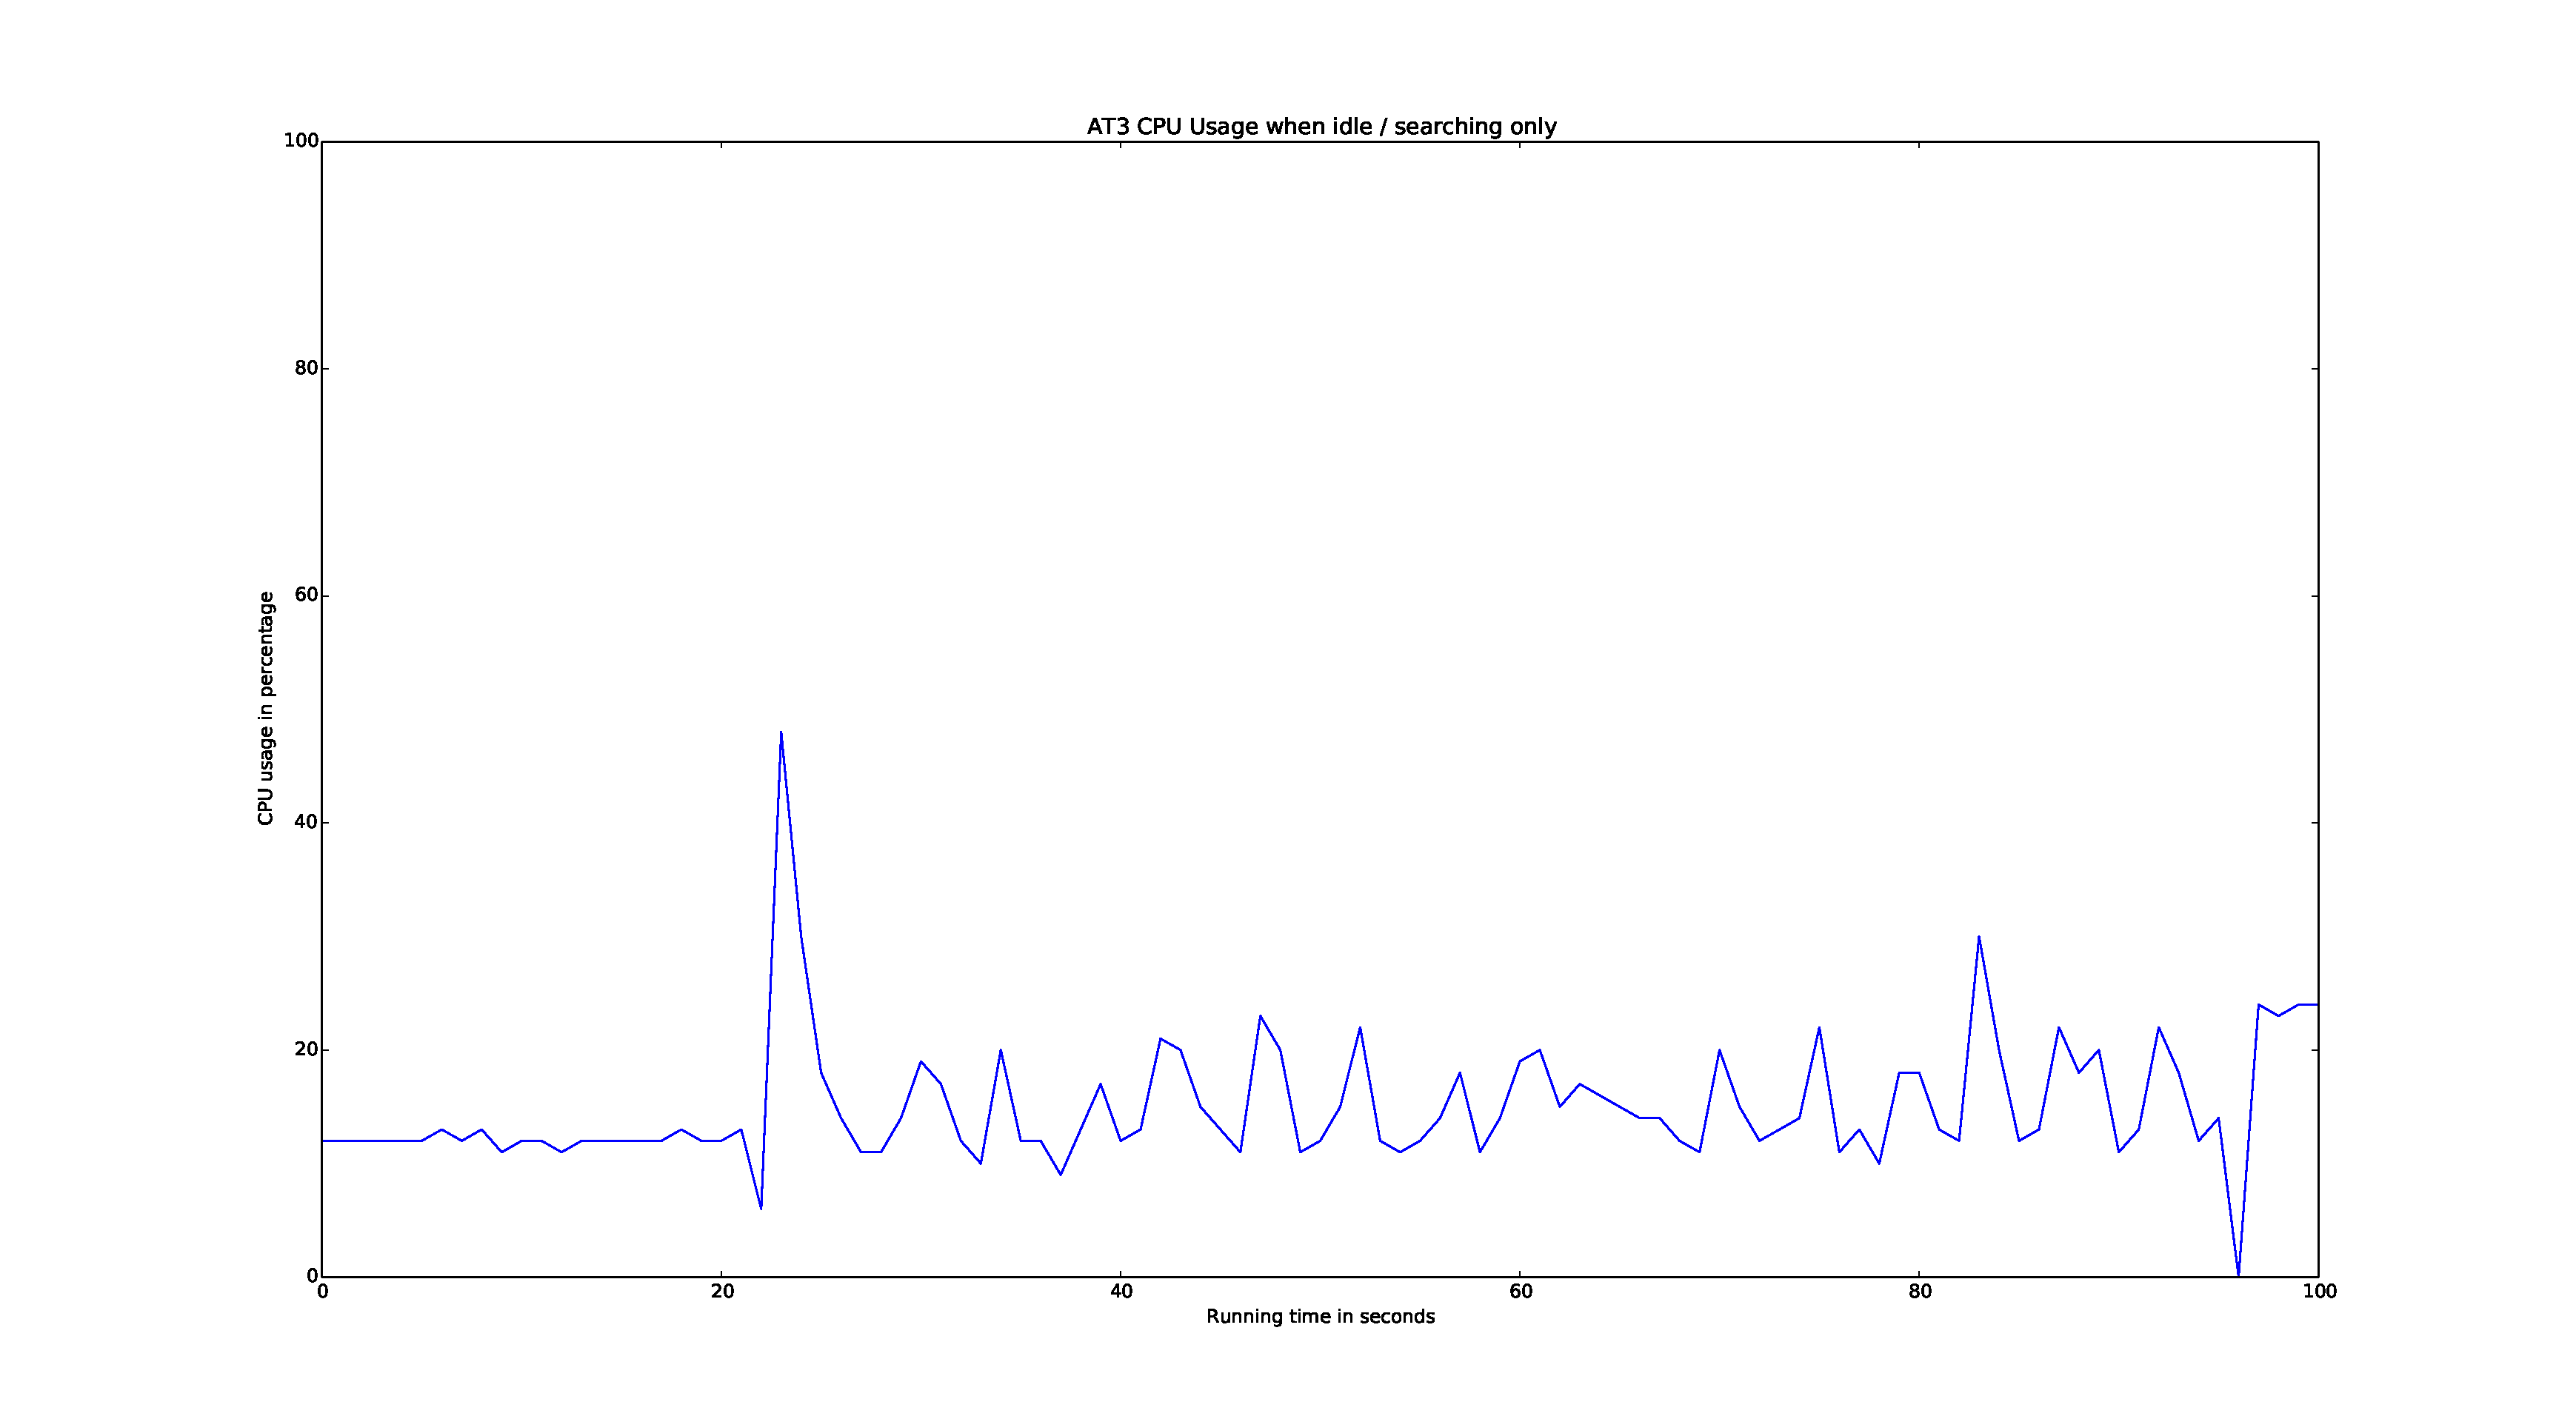
\includegraphics[width=\textwidth]{graphics/cpu_idle.pdf}
			\caption{The CPU usage of AT3 when in the idle state.}
			\label{fig:cpu_idle_graph}
		\end{figure*}
		
	\subsection{CPU usage with a direct download}
		When downloading the test file via a direct download, we see a stable, yet volatile CPU usage rate.
		These fluctuations seem natural as I/O operation are performed and other processes might require some time. 
		Figure \ref{fig:cpu_anonmode_off} shows the graph generated.
		
		\begin{figure*}[!htb]
			\centering
			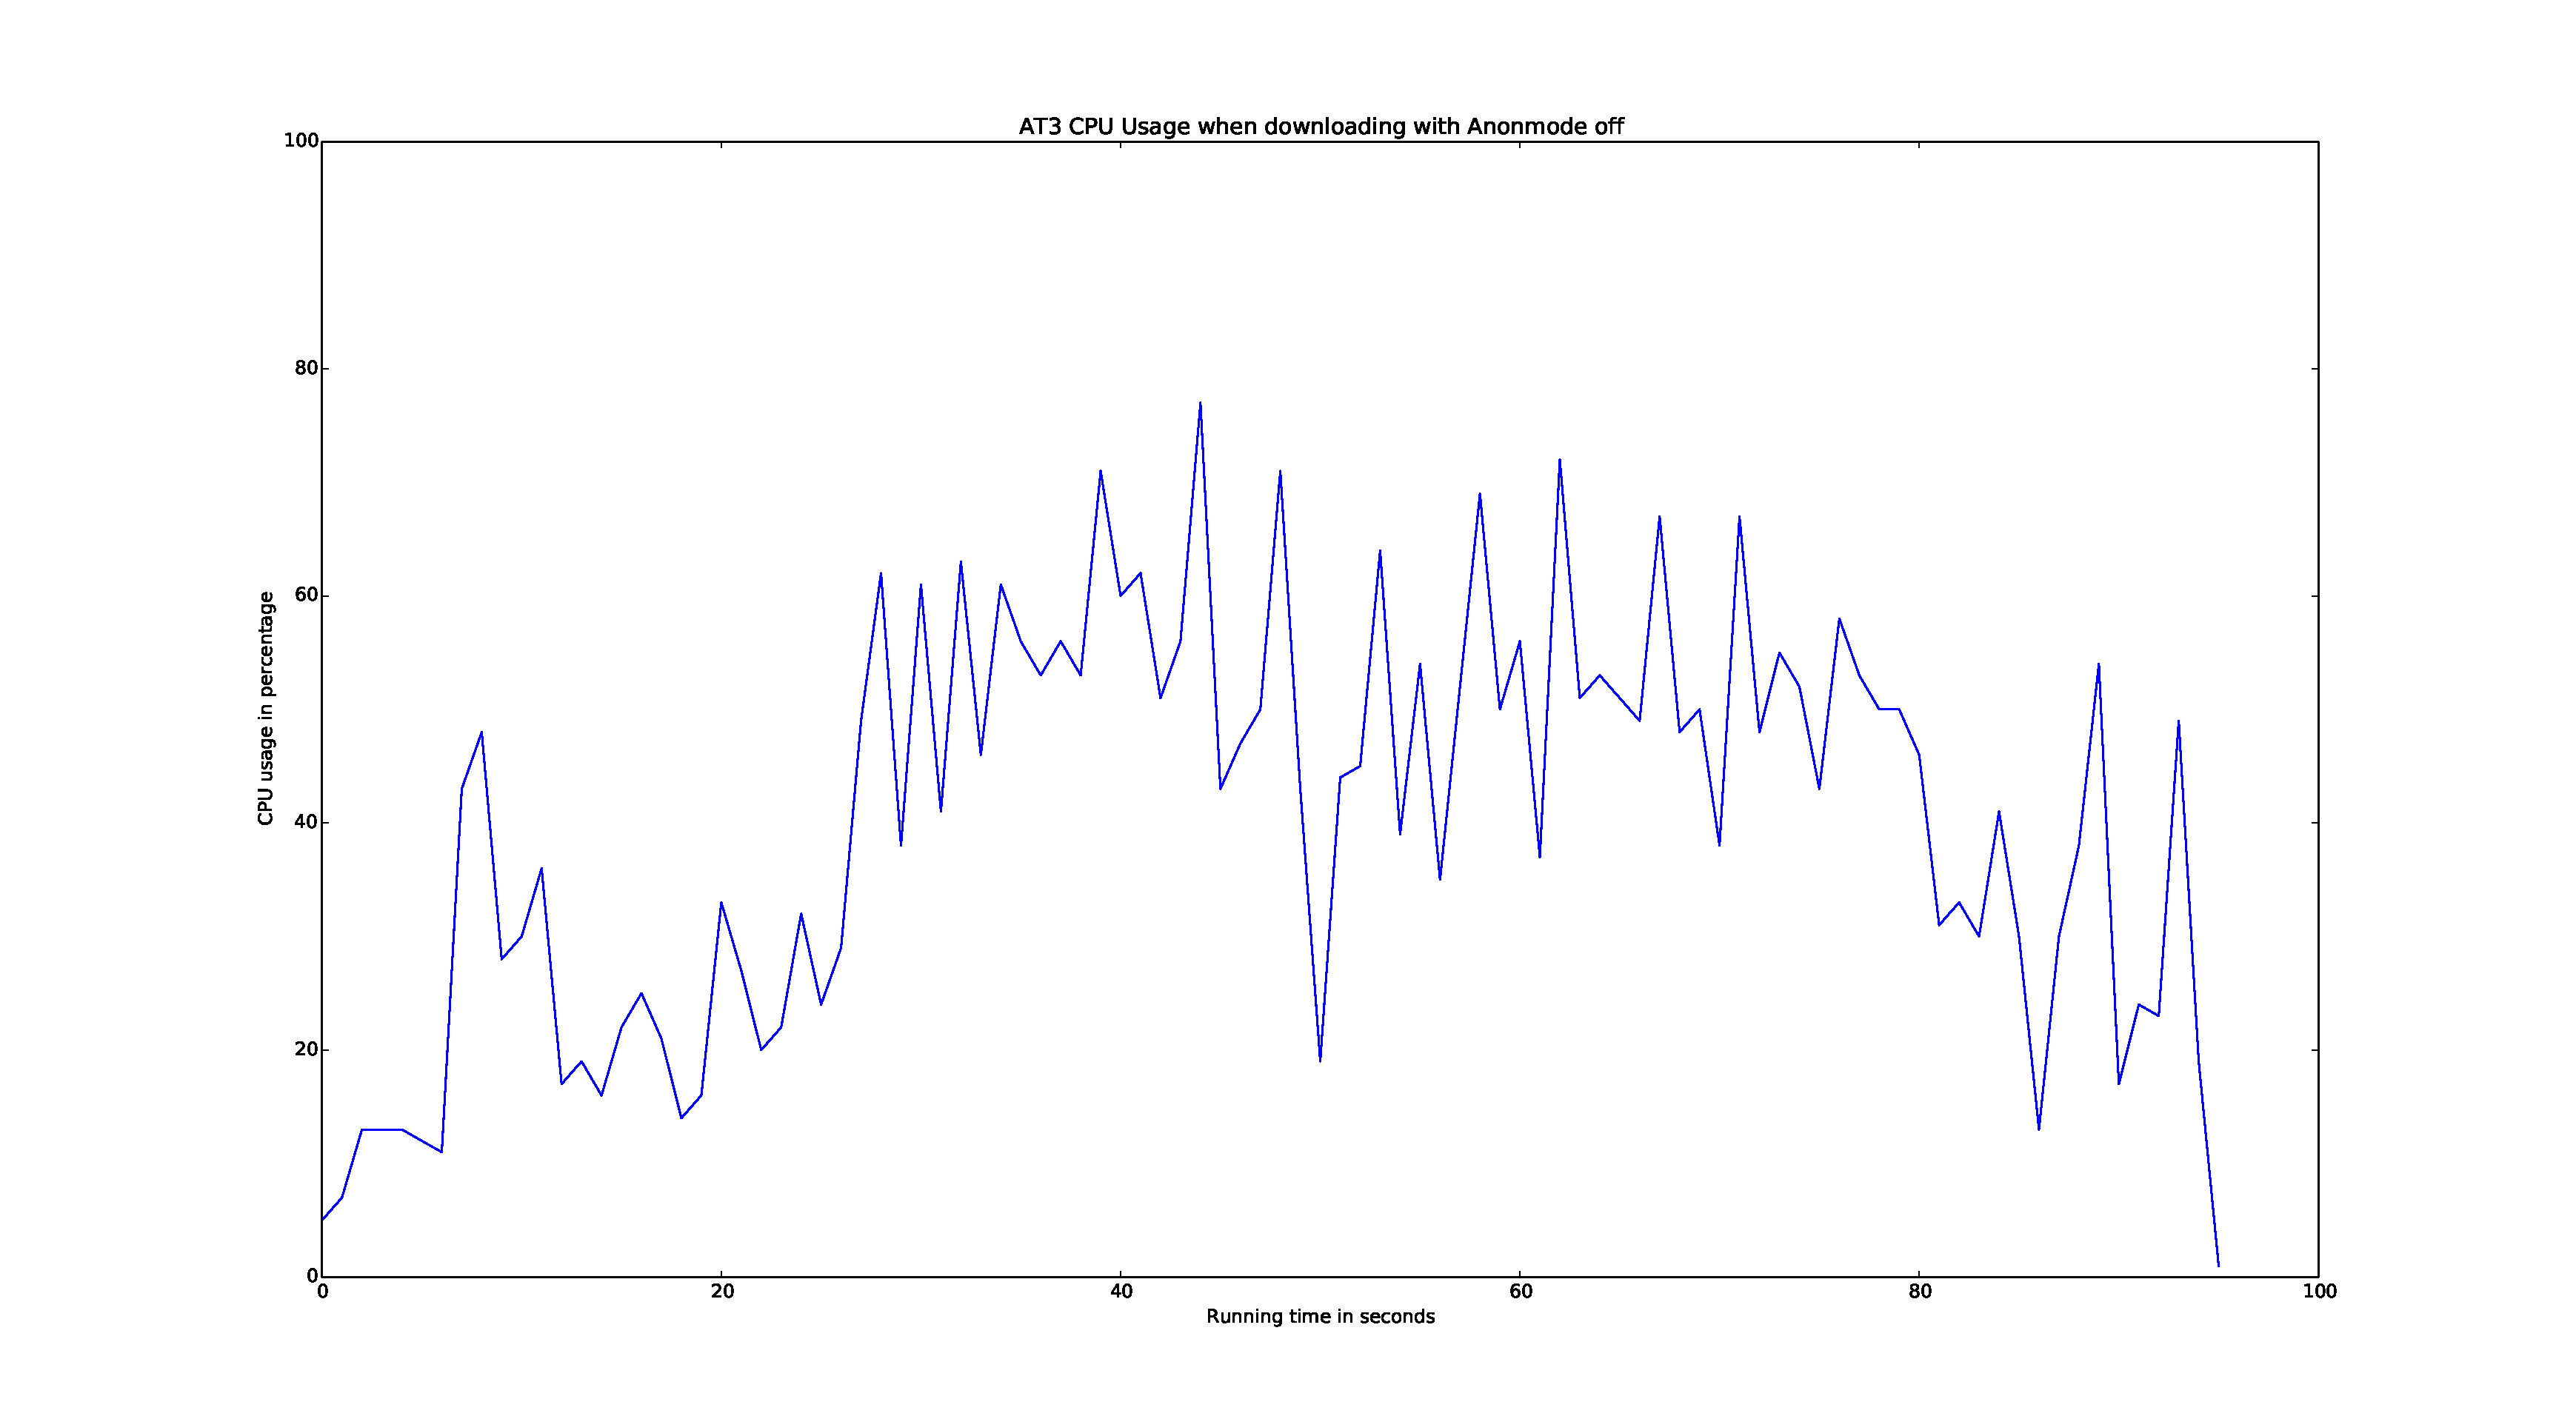
\includegraphics[width=\textwidth]{graphics/cpu_usage_anonmode_off.pdf}
			\caption{The CPU usage of AT3 when downloading directly.}
			\label{fig:cpu_anonmode_off}
		\end{figure*}
		
	\subsection{CPU usage when downloading with 1 hop and 1 circuit}
		When downloading the test file with 1 hop and 1 circuit, a raise in CPU usage is observed (see figure \ref{fig:cpu_1_hop_1_circuit}). The smartphone has to execute several cryptographic functions to decrypt the one layer of encryption on the data, which explains the raise. There is one drop which is also visible in the download rate graph of the download rate (figure \ref{fig:download_rate_1_hop_1_circuit}) where the application does not receive much data.
		The same peak in the idle graph is observed when the application starts up and creates a Tribler session.
		
		\begin{figure*}[!h]
			\centering
			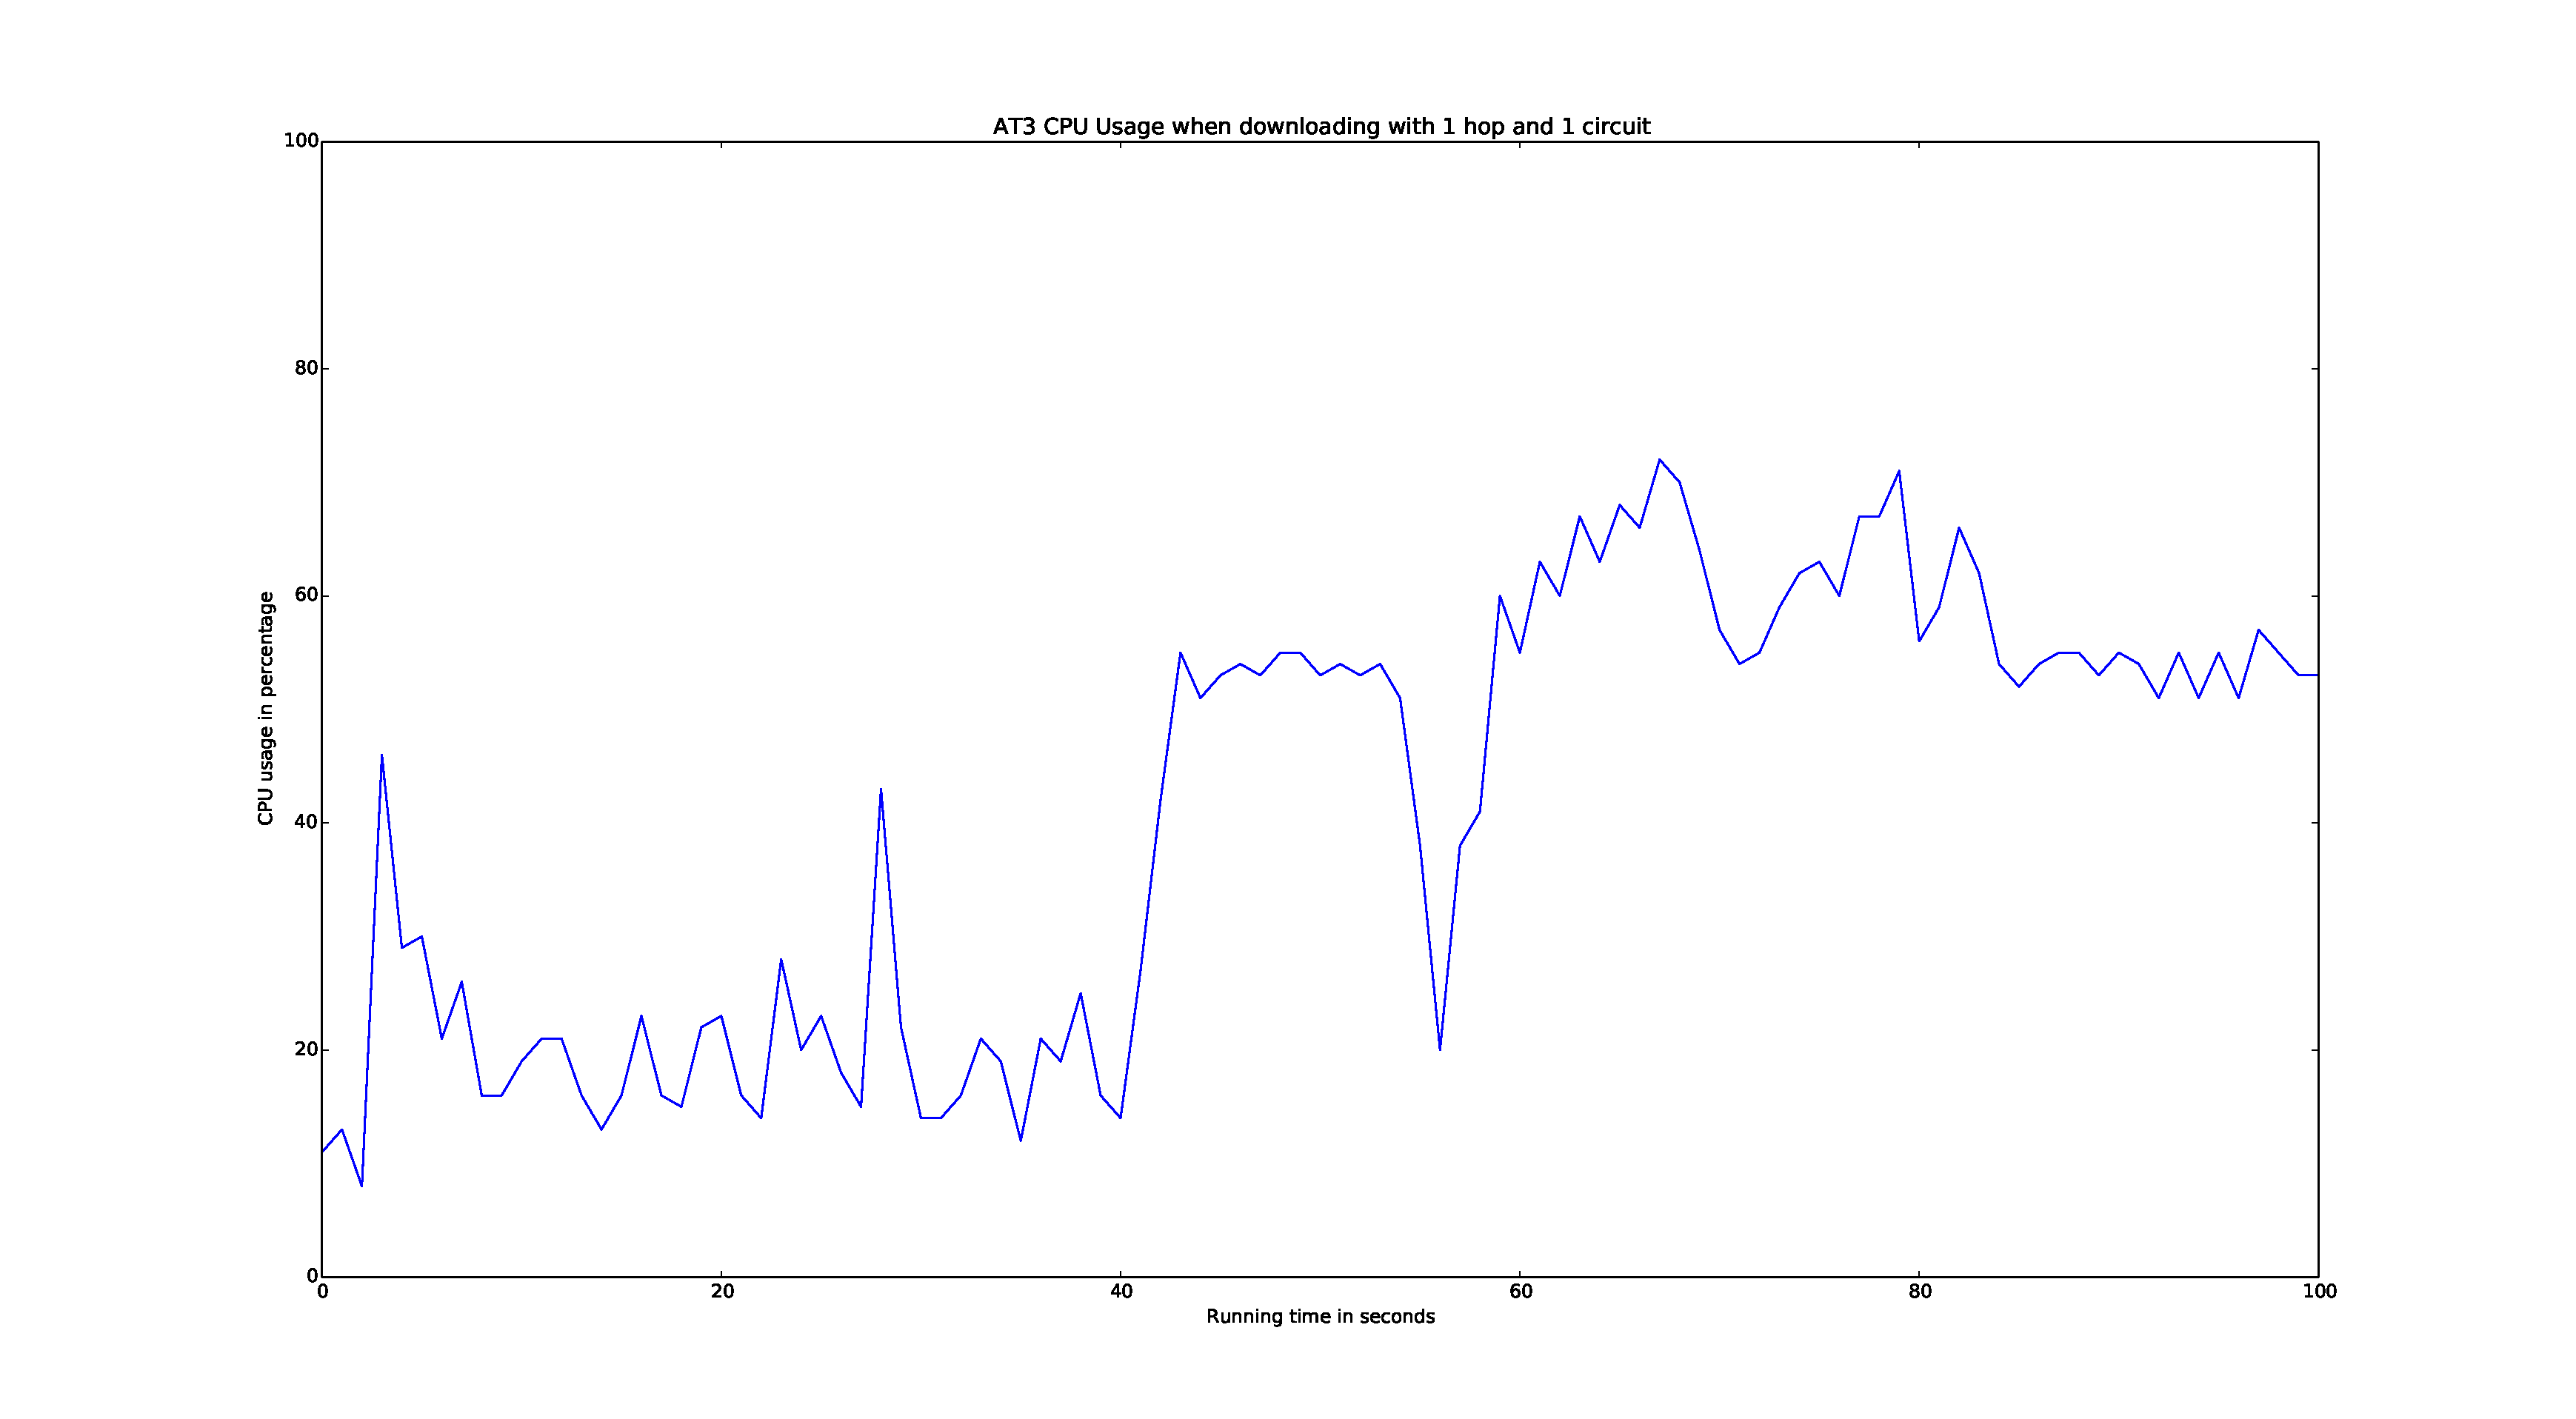
\includegraphics[width=\textwidth]{graphics/cpu_usage_1_hop_1_circuit.pdf}
			\caption{The CPU usage of AT3 when downloading over one hop and with one circuit.}
			\label{fig:cpu_1_hop_1_circuit}
		\end{figure*}
			
	\clearpage
	\subsection{CPU usage when downloading with 1 hop and 3 circuits}
		When we allow the anontunnel to download over two more circuits, we expect the CPU to raise a little more. The same cryptographic function has to be run, but at a possible higher rate per second. When we look at figure \ref{fig:cpu_1_hop_3_circuits}, we observe three peaks. We cannot explain these peaks exactly, but think it might be another process on the smartphone requiring CPU usage.
		
		\begin{figure*}[!h]
			\centering
			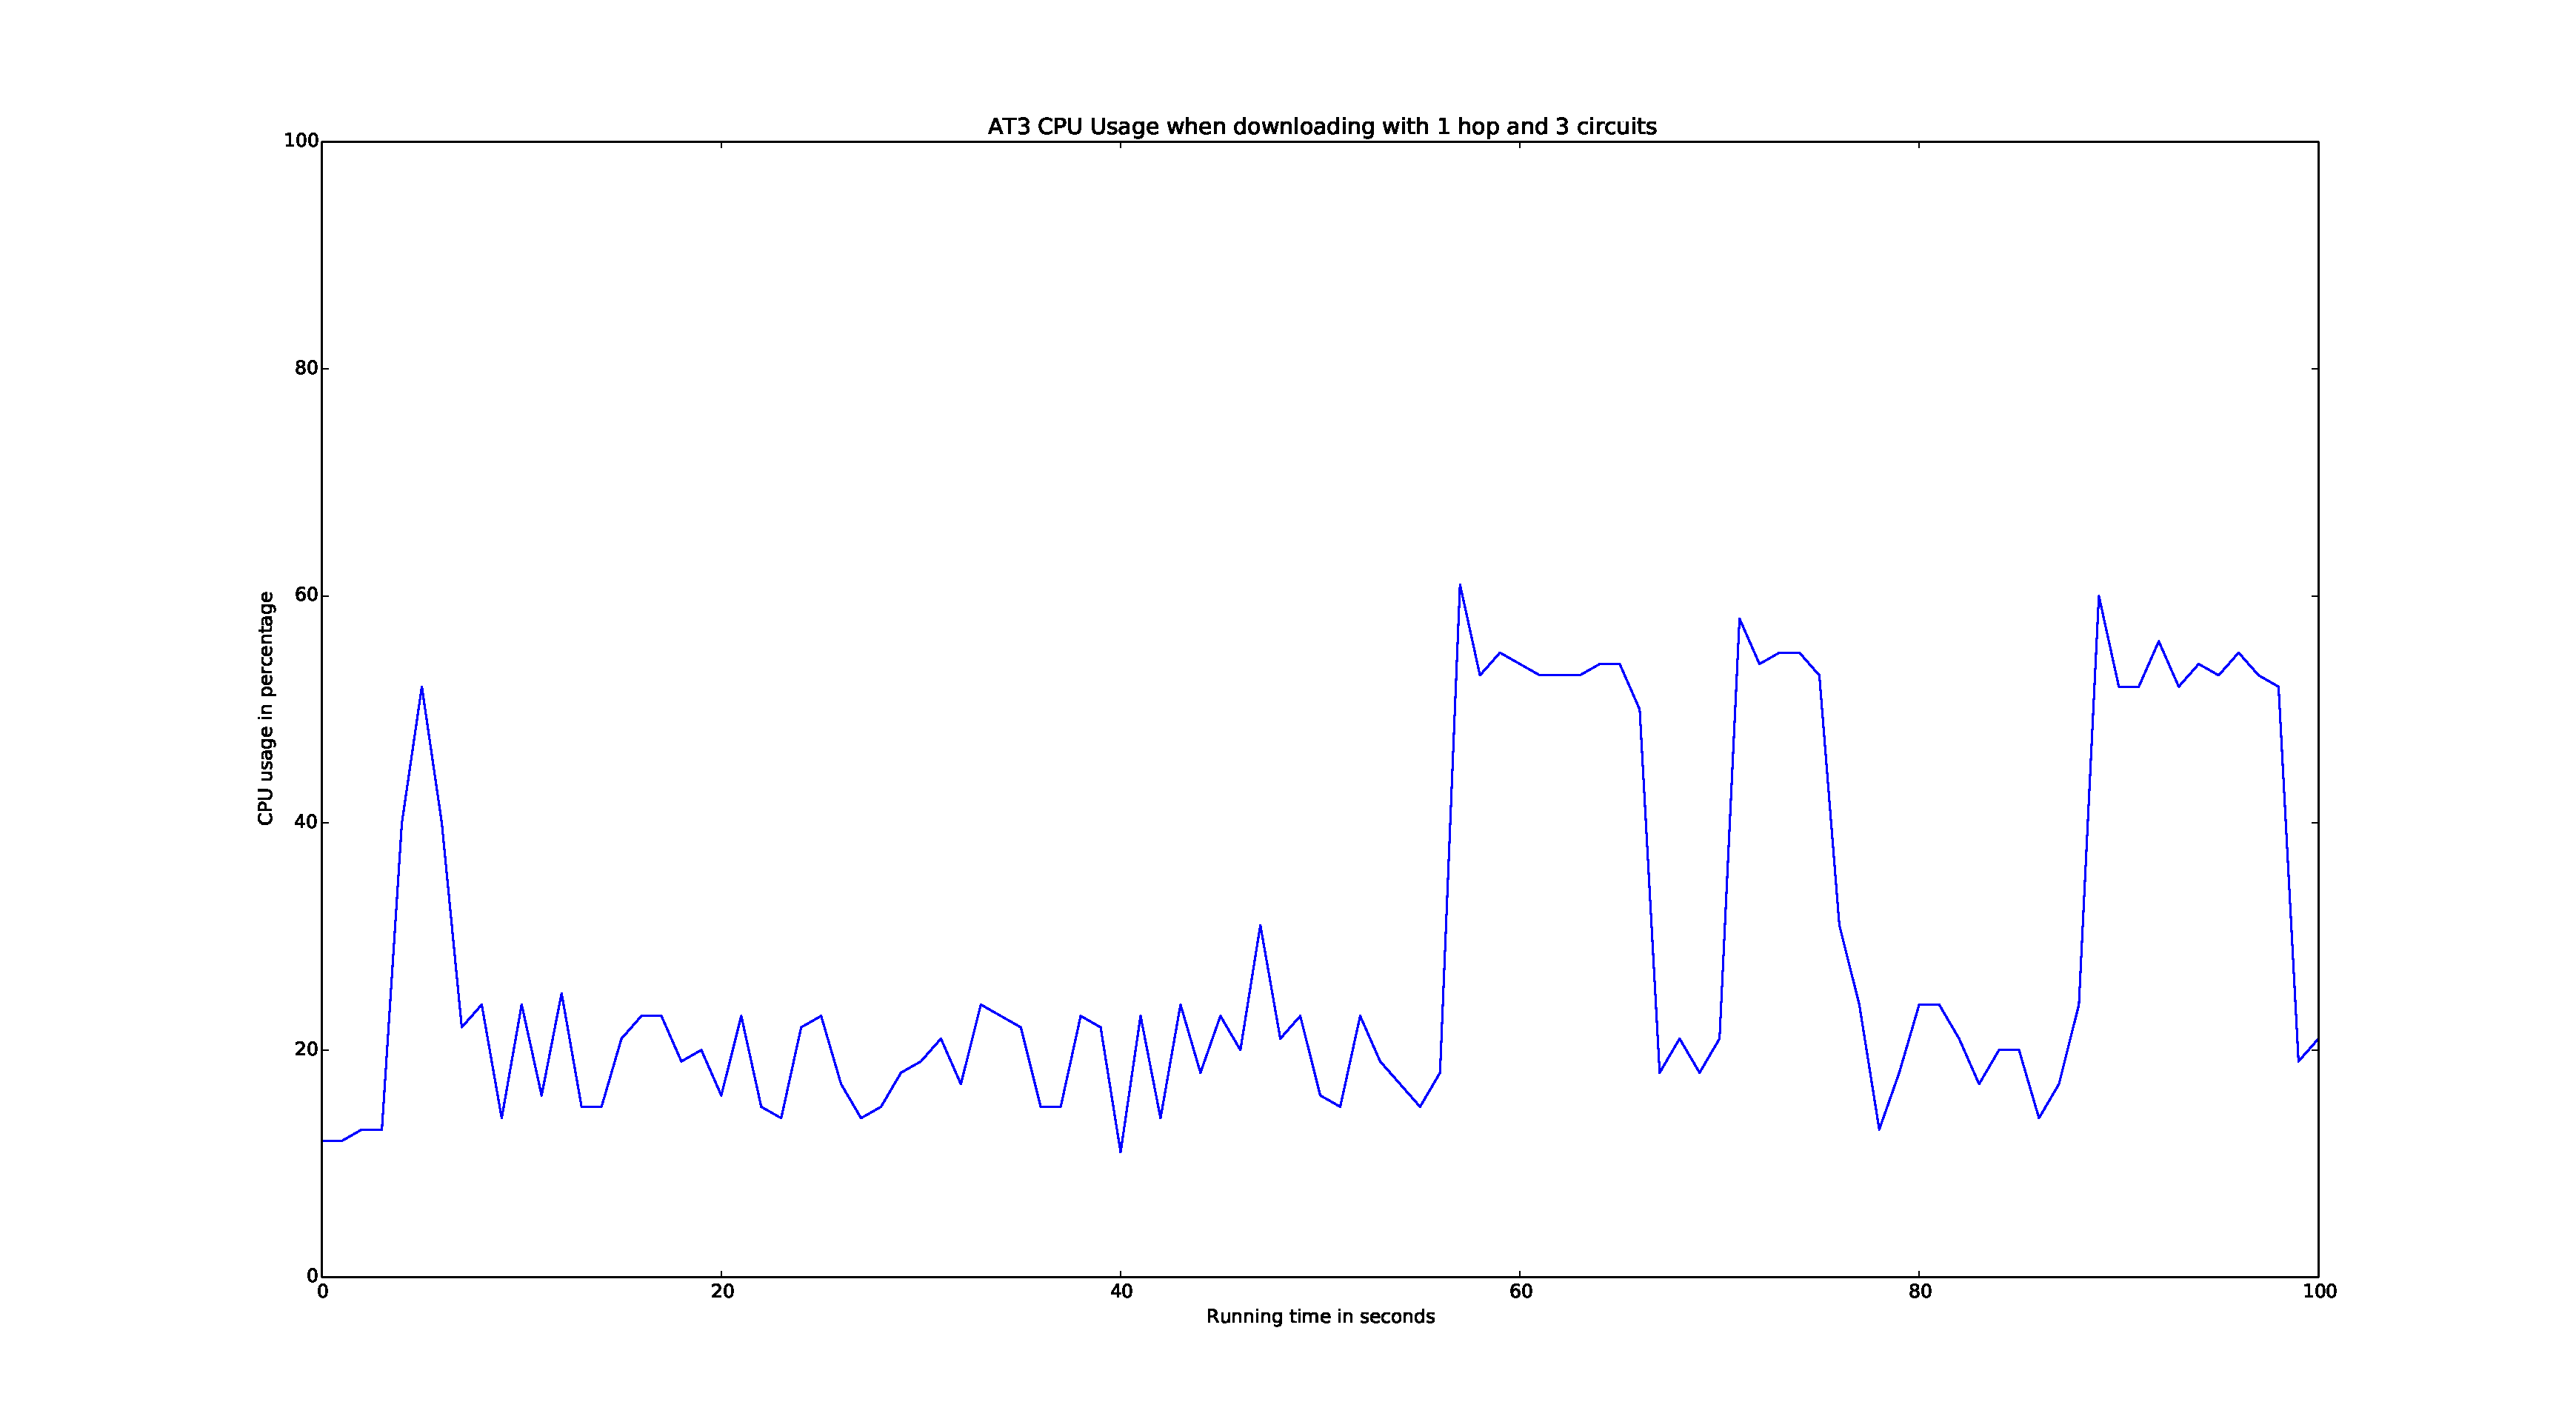
\includegraphics[width=\textwidth]{graphics/cpu_usage_1_hop_3_circuits.pdf}
			\caption{The CPU usage of AT3 when downloading over one hop and with three circuits.}
			\label{fig:cpu_1_hop_3_circuits}
		\end{figure*}
		
	\subsection{CPU usage when downloading with 3 hops and 1 circuit}
		\label{ssec:3_hops_1_circuit}
		When downloading with 3 hops we encountered a problem. As the device now has to encrypt / decrypt three layers, the CPU is heavily utilized by the cryptographic functions. The forming of circuits requires Diffie-Hellman handshakes and decrypting / encrypting packets prevents the mobile application to form any circuits. Before the connection can be established, the connection is timed out and the circuit is broken. This was both tested on a Google Nexus and a Sony Xperia Z.
		
		When we disable the encryption, circuits are formed in matter of seconds and the download is successfully completed.
		This means that the download was anonymous (unless the relays are malicious), but the data was not encrypted.
		
		Figure \ref{fig:cpu_3_hops_1_circuit} shows the graph generated of the three hops and 1 circuit with encryption disabled.
		
		\begin{figure*}[!h]
			\centering
			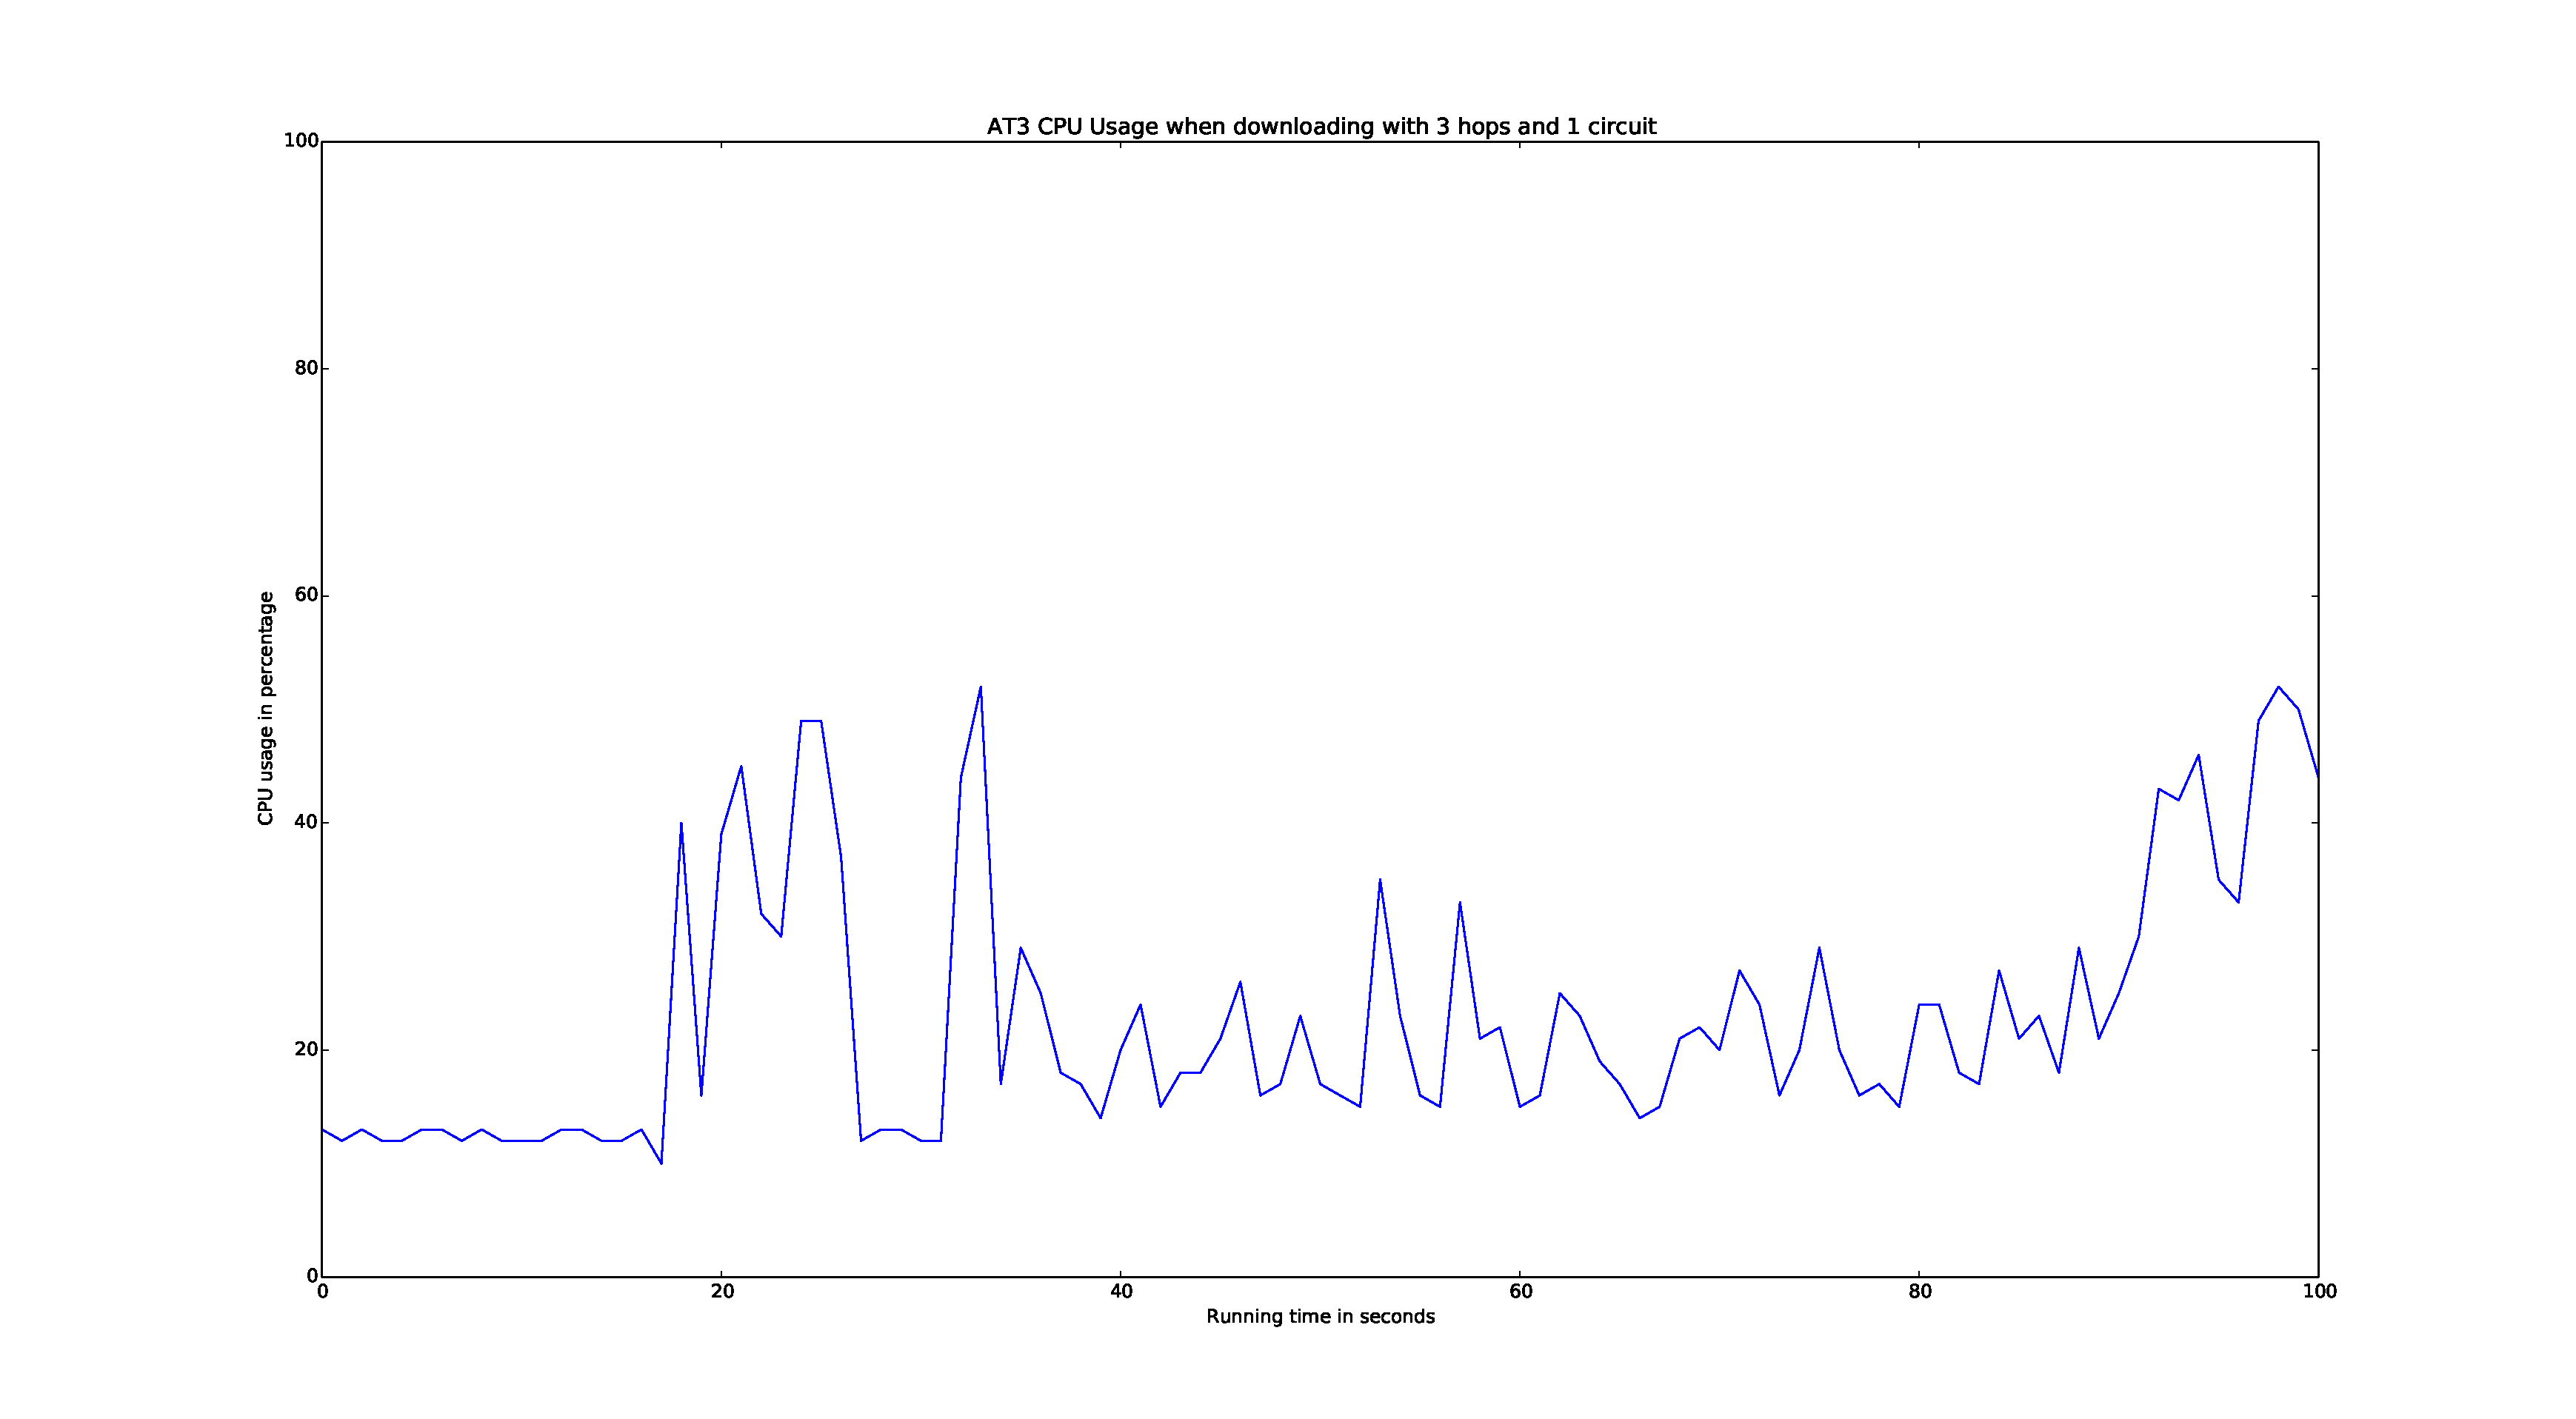
\includegraphics[width=\textwidth]{graphics/cpu_usage_3_hops_1_circuit.pdf}
			\caption{The CPU usage of AT3 when downloading over three hops and one circuit.}
			\label{fig:cpu_3_hops_1_circuit}
		\end{figure*}
		
	\subsection{CPU usage when downloading with 3 hops and 3 circuits}
		Since the issue of the CPU limit arose with just only one circuit, three circuits would not work either.
		Just to be sure, we also ran the test with 3 circuits, but to no avail. Circuits were not formed and the download did not start.
		
		When we disabled the crypto, we observed the same pattern as with the three hops and one circuit test. Circuits were made in seconds and the download soon started. The CPU of this run is visible in figure \ref*{fig:cpu_3_hops_3_circuits}.
		
		\begin{figure*}[!h]
			\centering
			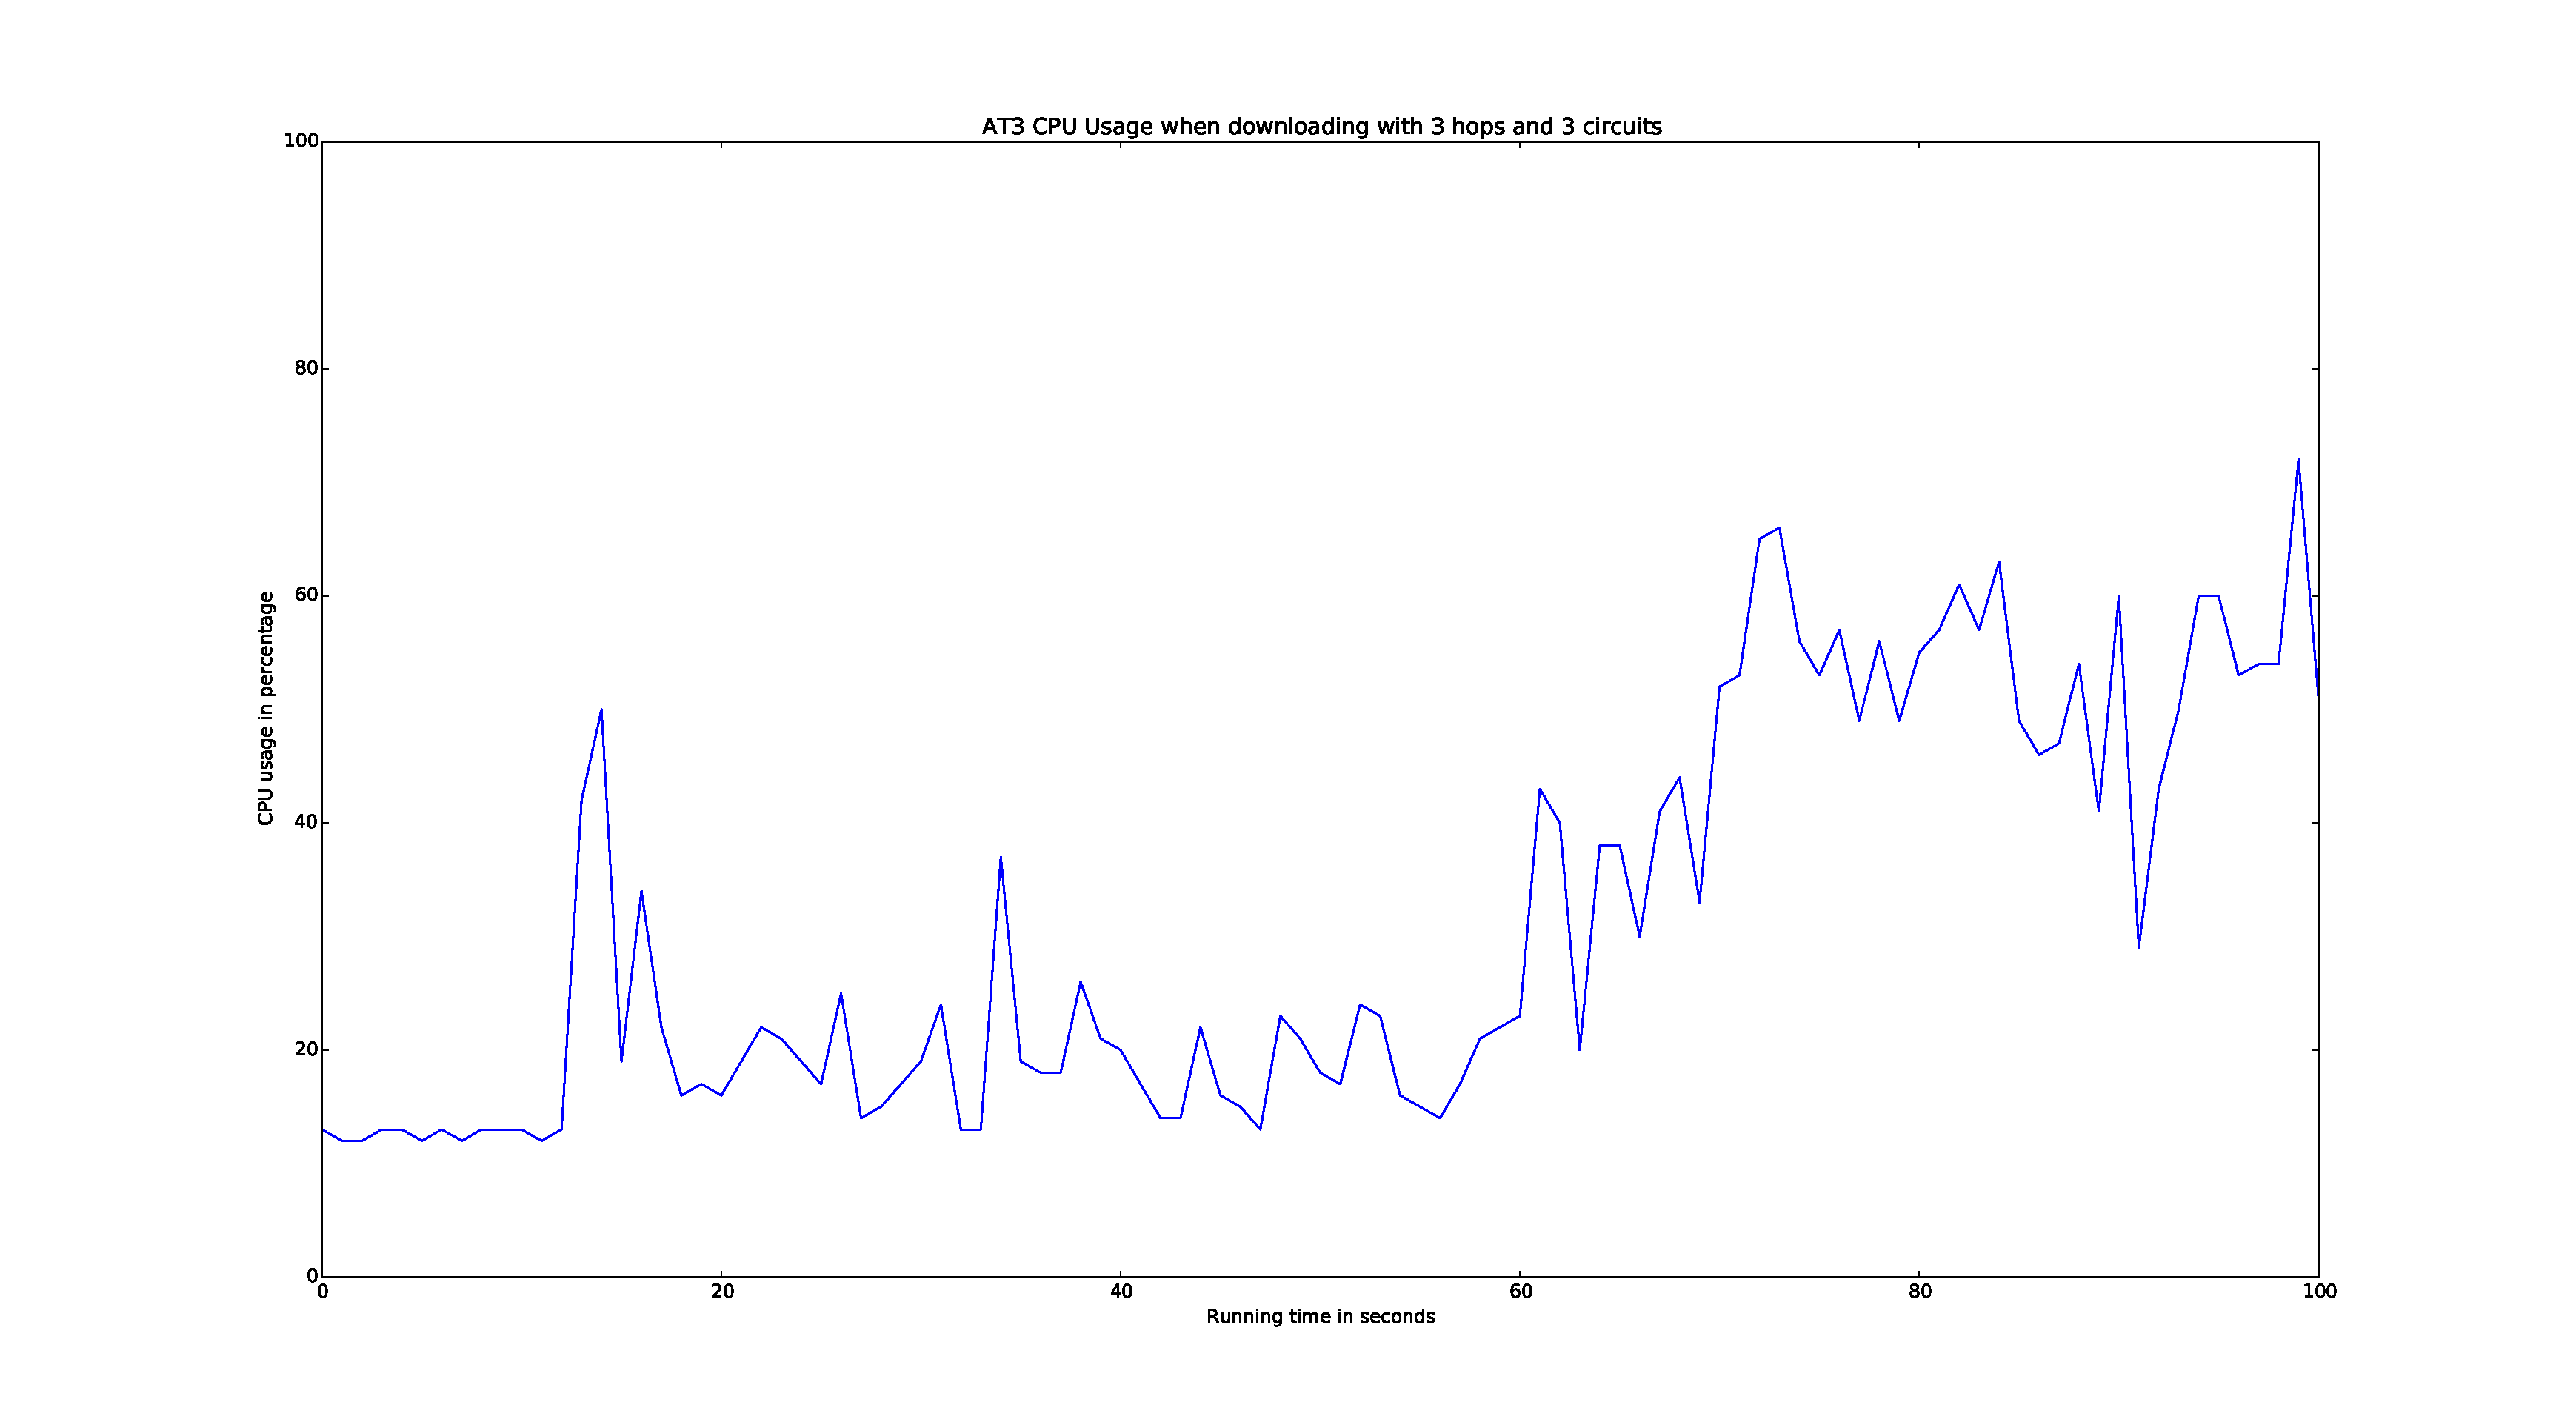
\includegraphics[width=\textwidth]{graphics/cpu_usage_3_hops_3_circuits.pdf}
			\caption{The CPU usage of AT3 when downloading over three hops and three circuits.}
			\label{fig:cpu_3_hops_3_circuits}
		\end{figure*}
		
\newpage